\section{Diseño base de datos}

{Dada la lógica y el diseño de la interfaz de usuario, se procede a crear la base de datos aplicando las reglas de normalización y así minimizar o evitar la redundancia de datos.

\begin{figure}[H]
	\centering
	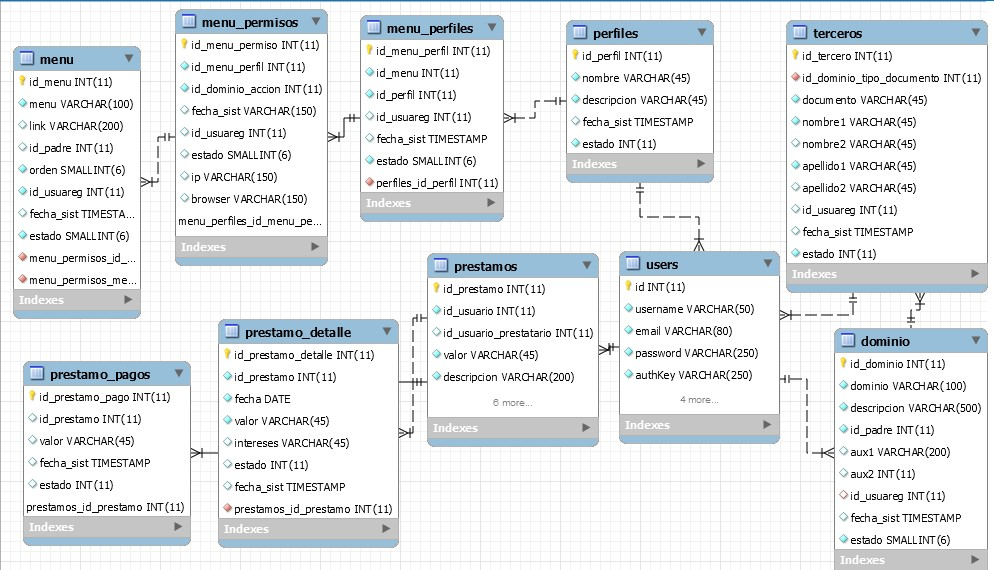
\includegraphics[width=1\linewidth]{development/modelo.png}
	\caption{Modelo relacional}
\end{figure}
\begin{center}
	\textbf{Fuente:} Propia.
\end{center}
}